%%%%%%%%%%%%%%%%%%%%%%%%%%%%%%%%%%%%%%%%%%%%%%%%%%%%%%%%%%%%%%%%%%%%
%% I, the copyright holder of this work, release this work into the
%% public domain. This applies worldwide. In some countries this may
%% not be legally possible; if so: I grant anyone the right to use
%% this work for any purpose, without any conditions, unless such
%% conditions are required by law.
%%%%%%%%%%%%%%%%%%%%%%%%%%%%%%%%%%%%%%%%%%%%%%%%%%%%%%%%%%%%%%%%%%%%

\documentclass[
  digital, %% The `digital` option enables the default options for the
           %% digital version of a document. Replace with `printed`
           %% to enable the default options for the printed version
           %% of a document.
%%  color,   %% Uncomment these lines (by removing the %% at the
%%           %% beginning) to use color in the printed version of your
%%           %% document
  oneside, %% The `oneside` option enables one-sided typesetting,
           %% which is preferred if you are only going to submit a
           %% digital version of your thesis. Replace with `twoside`
           %% for double-sided typesetting if you are planning to
           %% also print your thesis. For double-sided typesetting,
           %% use at least 120 g/m² paper to prevent show-through.
  lof,     %% The `lof` option prints the List of Figures. Replace
           %% with `nolof` to hide the List of Figures.
  lot,     %% The `lot` option prints the List of Tables. Replace
           %% with `nolot` to hide the List of Tables.
]{fithesis4}
%% The following section sets up the locales used in the thesis.
\usepackage[resetfonts]{cmap} %% We need to load the T2A font encoding
\usepackage[T1,T2A]{fontenc}  %% to use the Cyrillic fonts with Russian texts.
\usepackage[
  main=english, %% By using `czech` or `slovak` as the main locale
                %% instead of `english`, you can typeset the thesis
                %% in either Czech or Slovak, respectively.
  english, czech, slovak %% The additional keys allow
]{babel}        %% foreign texts to be typeset as follows:
%%
%%   \begin{otherlanguage}{czech}   ... \end{otherlanguage}
%%   \begin{otherlanguage}{slovak}  ... \end{otherlanguage}
%%
%% For non-Latin scripts, it may be necessary to load additional
%% fonts:
%\usepackage{paratype}
%\def\textrussian#1{{\usefont{T2A}{PTSerif-TLF}{m}{rm}#1}}
%%
%% The following section sets up the metadata of the thesis.
\thesissetup{
    date        = \the\year/\the\month/\the\day,
    university  = mu,
    faculty     = fi,
    type        = bc,
    department  = Department of Computer Systems and Communications,
    author      = Filip Karniš,
    gender      = m,
    advisor     = {RNDr. Miloš Liška, Ph.D.},
    title       = {Shongo Reservation System Backend REST API},
    TeXtitle    = {Shongo Reservation System Backend REST API},
    keywords    = {Shongo, REST, API},
    TeXkeywords = {Shongo, REST, API},
    abstract    = {%
      This is the abstract of my thesis, which can

      span multiple paragraphs.
    },
    thanks      = {%
      These are the acknowledgements for my thesis, which can

      span multiple paragraphs.
    },
    bib         = bibliography/example.bib,
    %% Remove the following line to use the JVS 2018 faculty logo.
    facultyLogo = fithesis-fi,
}
\usepackage{makeidx}      %% The `makeidx` package contains
\makeindex                %% helper commands for index typesetting.
% \usepackage[acronym]{glossaries}          %% The `glossaries` package
% \renewcommand*\glspostdescription{\hfill} %% contains helper commands
% \loadglsentries{misc/abbreviations_and_glossaries}  %% for typesetting glossaries
% \makenoidxglossaries                      %% and lists of abbreviations.
%% These additional packages are used within the document:
\usepackage{paralist} %% Compact list environments
\usepackage{amsmath}  %% Mathematics
\usepackage{amsthm}
\usepackage{amsfonts}
\usepackage{url}      %% Hyperlinks
\usepackage{markdown} %% Lightweight markup
\usepackage{listings} %% Source code highlighting
\lstset{
  basicstyle      = \ttfamily,
  identifierstyle = \color{black},
  keywordstyle    = \color{blue},
  keywordstyle    = {[2]\color{cyan}},
  keywordstyle    = {[3]\color{olive}},
  stringstyle     = \color{teal},
  commentstyle    = \itshape\color{magenta},
  breaklines      = true,
}
\usepackage{floatrow} %% Putting captions above tables
\floatsetup[table]{capposition=top}
\usepackage[babel]{csquotes} %% Context-sensitive quotation marks
\usepackage{hyperref}
\usepackage{cleveref}

%% Scales graphics to max \textwidth.
\newlength{\imgwidth}
\newcommand\scalegraphics[3]{
    \settowidth{\imgwidth}{\includegraphics{#1}}
    \setlength{\imgwidth}{\minof{\imgwidth}{\textwidth}}
    
    \begin{figure}[!ht]
      \centering
      \caption{#2}
      \includegraphics[width=\imgwidth]{#1}%
      \label{fig:#3}
    \end{figure}
}

\begin{document}
%% Uncomment the following lines (by removing the %% at the beginning)
%% and to print out List of Abbreviations and/or Glossary in your
%% document. Titles for these tables can be changed by replacing the
%% titles `Abbreviations` and `Glossary`, respectively.
% \clearpage
% \printnoidxglossary[title={Abbreviations}, type=\acronymtype]
% \printnoidxglossary[title={Glossary}]

%% The \chapter* command can be used to produce unnumbered chapters:
\chapter*{Introduction}
%% Unlike \chapter, \chapter* does not update the headings and does not
%% enter the chapter to the table of contents. I we want correct
%% headings and a table of contents entry, we must add them manually:
\markright{\textsc{Introduction}}
\addcontentsline{toc}{chapter}{Introduction}

Videoconferences have become a big topic in the last few years. With the globalization of the companies and an increasing number of people working remotely, the demand for methods that can be used for remote communication is growing in direct proportion.
Especially now, when the world pandemic stormed the lives of all mankind and limited the physical contact between people, they can appreciate the impact of this technology. The children and students can learn from their homes by communicating with their teachers \enquote{live} in the videoconferences mentioned earlier. Jobs that require communication considerably but do not require human contact can take full advantage of this technology.
However, the technology is bound to the available resources used for the videoconferences.

The academic community, as well as any large company, has a certain amount of resources at its disposal. For effective usage, the management of these resources is required.
For this purpose, the CESNET association created the Shongo system. The Shongo system manages available resources, makes reservations for these resources, and notifies participants about an upcoming videoconference.

This thesis was assigned to implement REST API for the Controller module (\Cref{controller}) of the Shongo system. The rest of the introduction focuses on describing this work's chapters.

In \Cref{cha:shongo}, the current reservation system Shongo will be introduced. Furthermore, this chapter discusses the current state of the Shongo architecture, its flaws, and how the architecture will change after the work on this thesis is done.

Next, the technologies used to finalize the assignment of this thesis have to be adequately explained. This explanation and a brief introduction to RESTful API can be found in \Cref{cha:technologies}.

When the reader is acquainted with the technologies used, the thesis continues to explain how they were used to complete the assignment in \Cref{cha:implementation}. This chapter describes the structure of the code added to the Shongo system --- the configuration, implementation and documentation of the REST API as the assignment requests.

Last but not least, the final API is described in \Cref{cha:api}, so the reader can imagine how the client can use the implemented REST API to interact with the Shongo system described in \Cref{cha:shongo}.

Finally, \Cref{cha:conclusion} summarizes the thesis and presents the thoughts about what can be done next.

\chapter{Reservation system Shongo}
In this chapter, we will introduce the reservation system Shongo for which this thesis will make \hyperref[rest]{REST API} extension.

Currently, at version v0.9.3, Shongo is a generic system used for managing resources.
Its primary function is to manage resources reservations for virtual meetings and any physical resources, such as physical meeting rooms, vehicles or parking places.
It allows administrators to define available resources (e.g., H.323 MCU or Adobe
Connect Server) and users to reserve the resources mentioned before. \cite{shongo}

CESNET association develops the system as an open-source project available at \href{https://github.com/shongo/shongo}{Github repository}, and it is currently deployed in these domains:
\begin{itemize}
    \item \url{https://meetings.cesnet.cz} - reservation system for H.323/SIP and Adobe Connect virtual rooms within CESNET videoconferencing infrastructure
    \item \url{https://meetings.cesnet.cz/ceitec} - reservation system for physical rooms of CEITEC - Central European Institute of Technology
    \item \url{https://meetings.cesnet.cz/cuni/} - reservation system for users led in authentication system of Charles University \footnote{\url{https://cuni.cz/}}.
\end{itemize}

Users can log in using their profile from any organization belonging to the Czech academic identity federation \footfullcite{eduid}.
After logging in, they can freely use the system and request reservations for available resources.

\enquote{CESNET is an association of universities and the Academy of Sciences of the Czech Republic that operates and develops a national e-infrastructure for science, research and education, including a computer network, computing grids, data repositories, collaborative environments and offering a wide range of services.} \cite{cesnet}

\section{Architecture}
% This section is mostly referenced from another thesis \footfullcite{pavelka2016shongo}, my primary learning material for how the Shongo system works.
I have drawn information for this section from shongo api documentation \footfullcite{shongoapi} and another thesis \footfullcite{pavelka2016shongo}.

The system is composed of a few separate modules. Their interconnections are shown in \Cref{architecture}.
\begin{figure}[!ht]
  \centering
  \caption{Shongo architecture}
%   % generated by Plantuml 1.2018.13      
\definecolor{plantucolor0000}{RGB}{168,0,54}
\definecolor{plantucolor0001}{RGB}{254,254,206}
\definecolor{plantucolor0002}{RGB}{0,0,0}
\begin{tikzpicture}[yscale=-1
,pstyle0/.style={color=plantucolor0000,line width=1.0pt,dash pattern=on 5.0pt off 5.0pt}
,pstyle1/.style={color=plantucolor0000,fill=plantucolor0001,line width=1.5pt}
,pstyle2/.style={color=plantucolor0000,fill=plantucolor0000,line width=1.0pt}
]
\draw[pstyle0] (32pt,38.2969pt) -- (32pt,116.5625pt);
\draw[pstyle0] (94.6593pt,38.2969pt) -- (94.6593pt,116.5625pt);
\draw[pstyle1] (8pt,3pt) rectangle (53.6593pt,33.2969pt);
\node at (15pt,10pt)[below right,color=black]{Bob};
\draw[pstyle1] (8pt,115.5625pt) rectangle (53.6593pt,145.8594pt);
\node at (15pt,122.5625pt)[below right,color=black]{Bob};
\draw[pstyle1] (67.6593pt,3pt) rectangle (119.6357pt,33.2969pt);
\node at (74.6593pt,10pt)[below right,color=black]{Alice};
\draw[pstyle1] (67.6593pt,115.5625pt) rectangle (119.6357pt,145.8594pt);
\node at (74.6593pt,122.5625pt)[below right,color=black]{Alice};
\draw[pstyle2] (83.6475pt,65.4297pt) -- (93.6475pt,69.4297pt) -- (83.6475pt,73.4297pt) -- (87.6475pt,69.4297pt) -- cycle;
\draw[color=plantucolor0000,line width=1.0pt] (32.8296pt,69.4297pt) -- (89.6475pt,69.4297pt);
\node at (39.8296pt,52.2969pt)[below right,color=black]{hello};
\draw[pstyle2] (43.8296pt,94.5625pt) -- (33.8296pt,98.5625pt) -- (43.8296pt,102.5625pt) -- (39.8296pt,98.5625pt) -- cycle;
\draw[color=plantucolor0000,line width=1.0pt,dash pattern=on 2.0pt off 2.0pt] (37.8296pt,98.5625pt) -- (94.6475pt,98.5625pt);
\node at (49.8296pt,81.4297pt)[below right,color=black]{Ok};
\end{tikzpicture}

%   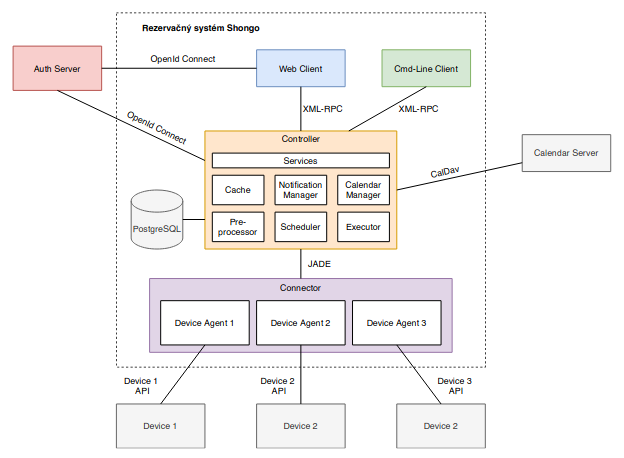
\includegraphics{assets/architecture}
  \makebox[\textwidth]{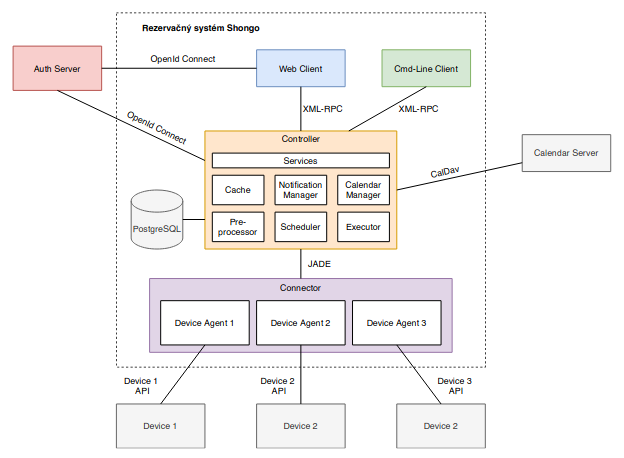
\includegraphics[width=\paperwidth]{assets/architecture}}
  \label{architecture}
\end{figure}

\subsection{Controller} \label{controller}
The controller module is the heart of the Shongo system. Its primary role is to plan requested reservations (\emph{Scheduler} sub-component) and assign necessary resources to them. Its secondary roles are informing users about their reservations (\emph{NotificationManager} sub-component) and administrate remote virtual resources (\emph{Executor} sub-component) via connected \hyperref[connector]{connectors}. Furthermore, last but not least, save this information to the relational database \emph{PostgreSQL}.

These functionalities are made available for other components with the \emph{Application programming interface} (API) via protocol \emph{XML-RPC}.

\subsection{Connector} \label{connector}
Connector is component that enable users to connect to video rooms with their devices (PC, tablet, smartphone, ...).

It is responsible for establishing, maintaining and monitoring connections with remote virtual resources.
It contains implementations for \emph{Device Agent}s where each \emph{Device Agent} can mediate a specific device (e.g. Adobe Connect, Pexip) functions to the controller using the device's API.
The controller communicates with the connector using the JADE (Java Agent DEvelopment) framework, which enables the connection of multiple connectors to a single controller.

\subsection{Authentication server}
The authentication server authenticates incoming requests for the controller component, authenticates users, finds users from various identity providers and gets information about users for the web client.
Besides that, it also manages the authentication layer of the web conference system Adobe Connect. This layer uses the user's information gained after logging in via system Shibboleth \footnote{Shibboleth, \url{https://www.shibboleth.net/}}.

\subsection{Web client} \label{webclient}
The web client is the system's primary interface for users. Using frameworks \emph{SpringMVC} and \emph{AngularJS}, it generates web pages with data gained from the controller's services.

Thanks to this component, users can authenticate via OpenID Connect \footnote{OpenID Connect, \url{https://openid.net/connect/}} and request a reservation for any available resource comfortably via the web.

\subsection{Command line client}
The command line client is the controller's additional interface used for administration. It enables system administrators to manage resources, user, groups and reservation requests which is not possible using the web client.

\section{What to Change and Why}

The main reason for changes is that the architecture concentrates on modularity; however, the system cannot be observed or managed from external sources.
The second reason is the primary user interface --- the \hyperref[webclient]{\emph{Web Client}} --- and its server-side rendering, which is not as powerful as today's JavaScript frameworks like Angular or React.
That is why developing a new front-end became a goal of another thesis \cite{drobnakm}.
Nevertheless, until now, the whole communication within the system has been done via Spring Framework in Java. In order to achieve communication between Shongo and the new Web Client (and possibly other systems or services), which is not part of the Shongo system, a new API has to be implemented.

\scalegraphics{assets/shongo_architecture_new_200}{New Shongo architecture}{architecture_new}

Comparing the old system architecture shown in \Cref{fig:architecture} and the new architecture shown in \Cref{fig:architecture_new} reveals that the \emph{Web Client} component was moved out of the Shongo system. The new \emph{Web Client} is now developed and maintained separately at the new Github repository\footnote{\url{https://github.com/shongo/shongo-frontend}}. Another thesis was devoted to this part of the changes \cite{drobnakm}.
Additionally, the \emph{Web Client} communicates with the \hyperref[controller]{\emph{Controller}} via \emph{HTTP} requests for the \emph{REST API} server sub-component instead of previous direct communication via \emph{XML-RPC} services. The implementation of said \emph{REST API} is the subject of this thesis.

\chapter{Used Technologies}
In this chapter, we will introduce the technologies that were used to do this work.

\section{Spring Framework} \label{sec:spring}
The Shongo system is written in Java. And the Spring Framework was used to develop it. \cite{spring}
The Spring Framework is. \cite{walls2022spring}

\section{Representational State Transfer} \label{rest}
Representational State Transfer or \texttt{REST} is an architectural style for distributed hypermedia systems. \cite{fielding2000rest}
\subsection{REST design principles}
Unlike other API designs such as XML-RPC or SOAP, REST APIs can developed using virtually any language and support any format for communication. However, there is a set of rules that has to be followed in order to call it a REST API.

These rules are called REST design principles --- also known as architectural constraints:
\cite{ibmrest}
\begin{enumerate}
    \item \textbf{Uniform interface} -- all API requests for the same resource should have a same form disregards of what is the request origin. Same piece of data, such as name or email of a user, belongs to one uniform URI (uniform resource identifier).
    \item \textbf{Client-server decoupling} -- client and server side of application should be completely independent of each other. Client should have only one information --- the URI of requested resource. Meaning it cannot interact with server in any other ways. Analogically the server should affect the client in no other way than passing requested data to it.
    \item \textbf{Statelessness} -- each request has to include all the information needed to processing it. Meaning that server is not allowed to store any data related to request and there are no server-side sessions.
    \item \textbf{Cacheability} -- as low as possible requests should be made to reduce traffic and improve performance, so as many as possible resources should be cacheable. Server should also inform client whether given data in response is suitable for caching.
    \item \textbf{Layered system architecture} -- requests and responses can go through many layers on their way. There may be a number of different intermediaries in the communication. As a result neither server nor client can assume that they are communicating directly with application or with an intermediary.
    \item \textbf{Code on demand (optional)} -- in some cases the response can be executable code (Java applets for example). In these cases, the code should only run on-demand.
\end{enumerate}

\section{OpenAPI} \label{sec:openapi}

\section{Swagger} \label{sec:swagger}
The Swagger is the most used modern way to document REST APIs.
\cite{swagger}

\section{Mockoon} \label{sec:mockoon}

\section{Postman} \label{sec:postman}

\section{Lombok} \label{sec:lombok}

\section{Jackson} \label{sec:jackson}
Jackson serializes classes using getters and deserializes using setters from JSON (JavaScript Object Notation), alternatively XML (Extensible Markup Language) or any other supported format.

\chapter{Implementation}
All classes related to the REST API are stored in the Controller’s package  \texttt{cz.cesnet.shongo.controller.rest}.
Aside from this package, the only changes made are in a few files that retrieve data from the database --- where additional data were required to be loaded --- and inter-domain implementation files\cite{pavelka2016shongo} whose configuration has been merged with the REST configuration.

\section{REST Server}
The cornerstone of the implementation is the REST server which listens for incoming HTTP requests from clients and responds to them in the desired way. The REST server is implemented in the \texttt{RESTApiServer} class.
At the start of the \emph{Controller} service, the REST server is attached to the \emph{Controller}.

\texttt{RESTApiServer} starts a \emph{Jetty}\footnote{\url{https://www.eclipse.org/jetty/}} server and configures it according to the controller configuration. The server then listens on the host and port specified in the configuration.

\section{Configuration}
The REST server configuration is required before implementing API endpoints. These configuration files are stored in the \texttt{config} sub-package.

\subsection{Configuration File Extension}
First, the configuration of the REST server itself is essential. The controller configuration file \texttt{shongo-controller.cfg.xml} has been extended with the parameterization for the new code. Thanks to that, Shongo administrators can set the REST API server properties inside the \texttt{<rest-api>} XML element. An example of this new configuration is shown in \Cref{conf}. There are several configurable sub elements:
\begin{itemize}
    \item \texttt{<host>} -- the host where the REST API shall serve
    \item \texttt{<port>} -- the port where the REST API shall serve
    \item \texttt{<ssl-key-store>} -- the SSL (Secure Socket Layer) key store
    \item \texttt{<ssl-key-store-type>} -- the type of key store
    \item \texttt{<ssl-key-store-password>} -- the password for key store
\end{itemize}

\begin{lstlisting}[language=XML, caption=REST configuration example, label=conf]
<?xml version="1.0" encoding="UTF-8" ?>
<configuration>
    ...
    <rest-api>
        <host>meetings.cesnet.cz</host>
        <port>9999</port>
        <ssl-key-store>keystore/server.keystore</ssl-key-store>
        <ssl-key-store-password>
            (password)
        </ssl-key-store-password>
    </rest-api>
    ...
</configuration>
\end{lstlisting}

\subsection{Security}
Next, the security and authentication had to be configured. For this purpose, \emph{Spring security} is used. Spring security dependencies have been added to \emph{Controller}'s \texttt{pom.xml}, and security configuration files were stored in \texttt{config.security} sub-package.

The web security is configured in the \texttt{SecurityConfig} class annotated with the Spring \texttt{@EnableWebSecurity} annotation, which allows this class to configure web security\cite{springdocumentation}.
This configuration file defines what should happen to the incoming request. The request filters are added to the request processing, and CORS (Cross-Origin Resource Sharing)\footnote{\url{https://www.w3.org/TR/cors/}} is configured here. The paths that should be skipped in the authentication process are also set here. At the moment, these include OpenAPI, Swagger, inter-domain endpoints\cite{pavelka2016shongo}, and endpoints responsible for processing problem reports.

Additionally, \texttt{AuthFilter} is added, which serves as a REST API middleware. It processes each request (omitting those configured in SecurityConfig) using the following steps:
\begin{enumerate}
    \item Decode an access token wrapped in the HTTP request authorization header as a bearer token.
    \item Check the token authorization.
    \item Convert the token into \texttt{SecurityToken} object which contains an \emph{access token} for Shongo Controller and cached information about the user to whom the token belongs.
    \item Add this new object to the request attributes using the \texttt{TOKEN} key so that subsequent endpoint handling (next middleware or final method) can effortlessly work with it.
\end{enumerate}
If the token is not present or is invalid, the server responds with an HTTP \emph{401 UNAUTHORIZED} response code.

\subsection{OpenAPI and Swagger}
The \hyperref[sec:openapi]{OpenAPI} specification is generated using Springdoc from the \hyperref[sec:spring]{Spring framework}, so the users can have general and straightforward API documentation available to them.
For this purpose, the \emph{springdoc-openapi} dependency was added to \emph{Controller}'s \texttt{pom.xml}, and the \texttt{OpenApiConfig} class was created. In this configuration file, Springdoc dependencies were imported using Spring's \emph{@Import}, global API attributes were defined with \texttt{@OpenAPIDefinition}, and security was defined with \texttt{@SecurityScheme} annotation.
This is shown in \Cref{lst:openapi}.
\begin{lstlisting}[language=Java, caption=OpenApiConfig.java, label=lst:openapi]
@Configuration
@EnableWebMvc
@OpenAPIDefinition(
        info = @Info(title = "Shongo API", version = "v1"),
        security = @SecurityRequirement(name = "bearerAuth")
)
@SecurityScheme(
        name = "bearerAuth",
        type = SecuritySchemeType.HTTP,
        scheme = "bearer"
)
@ComponentScan(basePackages = {"org.springdoc"})
@Import({
        SpringDocConfiguration.class,
        SpringDocWebMvcConfiguration.class,
        SwaggerConfig.class,
        SwaggerUiConfigProperties.class,
        SwaggerUiOAuthProperties.class,
        JacksonAutoConfiguration.class
})
class OpenApiConfig implements WebMvcConfigurer {
    ...
}
\end{lstlisting}
Springdoc generates OpenAPI specification based on Spring web annotations by default, but Springdoc annotations such as \texttt{@Operation} or \texttt{@ApiResponses} can customize the resulting specification.
The resulting OpenAPI file is added to the REST server and is available at the \texttt{/v3/open-api} path. \cite{springdoc}

The \hyperref[sec:swagger]{Swagger UI} is then used for user-friendly visualization of the documentation mentioned above.
The user interface (web site) is acquired and saved in the project resources using the same \emph{springdoc-openapi} dependency as for OpenAPI specification. After that, the default OpenAPI path is modified from \texttt{https://\-petstore.swagger.io\-/v2/swagger\-.json} to \texttt{/v3/open-api}. Finally, we add these resources to the REST API server and make them available at the  \texttt{/swagger-ui/index.html} path.

\section{REST Controllers}
This section uses information from Spring documentation \cite{springdocumentation}.
The REST Controllers are responsible for operating the API endpoints and are stored in the \texttt{controllers} sub-package. An example of such a Controller can be observed in \Cref{lst:controller}.

The REST Controllers are annotated with \texttt{@RestController} annotation from the Spring framework, which combines two other annotations:
\begin{description}
    \item \texttt{@Controller} -- makes the class auto-detectable through classpath scanning
    \item \texttt{@ResponseBody} -- binds the return values of the mapped methods to the HTTP response body
\end{description}
This annotation is combined with the \texttt{@RequestMapping} annotation, which uses the web request path to map the incoming request to the method that processes the request and responds to the client. \texttt{@RequestMapping} can also be parameterized, particularly with path (path to the endpoint), consumes (expected incoming body form), and produces (outgoing body form).

There are usually only a few attributes in the controller classes. These attributes are generally Controller’s services, and \emph{dependency injection} is used to access these services. Thanks to Spring annotation \texttt{@Autowired}, they are resolved to \emph{Beans} defined in \texttt{rest-api-servlet.xml} and injected into the controller class. The example of this file can be noticed in \Cref{lst:beans}.

\begin{lstlisting}[language=XML, caption=rest-api-servlet.xml, label=lst:beans]
<?xml version="1.0" encoding="UTF-8"?>
<beans xmlns=
"http://www.springframework.org/schema/beans"
       ...>
    <context:component-scan base-package="cz.cesnet.shongo.controller"/>
    <mvc:annotation-driven />
    <aop:aspectj-autoproxy />
    
    <bean id="controller" class=
    "cz.cesnet.shongo.controller.Controller" factory-method="getInstance"/>
    <bean id="configuration" factory-bean="controller" factory-method="getConfiguration"/>
    <bean id="controllerClient" class=
    "cz.cesnet.shongo.controller.ControllerClient">
        <constructor-arg>
            <bean factory-bean="configuration" factory-method="getRpcUrl"/>
        </constructor-arg>
    </bean>
    <bean id="controllerReservationService" factory-bean="controllerClient" factory-method="getService">
        <constructor-arg value=
        "cz.cesnet.shongo.controller.api.rpc.
        ReservationService" type="java.lang.Class"/>
    </bean>
    ...
    <bean id="cache" class=
    "cz.cesnet.shongo.controller.rest.Cache"/>
</beans>
\end{lstlisting}

The last part of REST Controllers is the declaration and implementation of methods handling distinct REST resources. The methods are annotated with \texttt{@RequestMapping} or rather an exact mapping according to the selected HTTP method (\texttt{@GetMapping}, \texttt{@PostMapping}, \texttt{@PutMapping}, \texttt{@DeleteMapping}).
These annotations also take a path parameter, which is then concatenated to the class’s \texttt{@RequestMapping} path parameter.
In addition, the methods can retrieve HTTP request attributes annotated with \texttt{@RequestAttribute} (most importantly SecurityToken added by AuthFilter), HTTP request parameters annotated with \texttt{@RequestParam}, path parameters annotated with \texttt{@PathVariable} (and specified in the path as \texttt{"\{variableName\}"}) and also body parameter annotated with \texttt{@RequestBody}.

\begin{lstlisting}[language=java, caption=ReservationRequestController.java, label=lst:controller]
// Makes this path a Controller (auto-detectable) and binds return values of methods to the HTTP request body
@RestController
// Binds this controller to the path parameter
@RequestMapping("/api/v1/reservation_requests")
public class ReservationRequestController
{
    // Controller service used to manage reservations
    private final ReservationService reservationService;
    
    // @Autowired resolves the service to Bean defined in rest-api-servlet.xml
    public ReservationRequestController(@Autowired ReservationService reservationService)
    {
        this.reservationService = reservationService;
    }
    
    // Binds this method to the HTTP GET request with path defined in @RequestMapping
    @GetMapping
    // Method returns ListResponse<ReservationRequestModel> in response body thanks to @RestController annotation
    ListResponse<ReservationRequestModel> listRequests(
        // Gets security token from request attributes. The token was stored there when AuthFilter processed the request.
        @RequestAttribute(TOKEN) SecurityToken securityToken,
        // Reads optional request parameter allocation_state and stores it in allocationState variable
        @RequestParam(value = "allocation_state", required = false) AllocationState allocationState,
        ...
    )
    {
        // Use Controller service to acquire requested data
        ReservationRequestListRequest request = new ReservationRequestListRequest();
        request.setAllocationState(allocationState);
        ...
        ListResponse<ReservationRequestSummary> response = reservationService.listReservationRequests(request);
        ...
        // Return the acquired data
        return response;
    }
    
    // Binds this method to the HTTP POST request with path defined in @RequestMapping
    @PostMapping
    void createRequest(
        @RequestAttribute(TOKEN) SecurityToken securityToken,
        // Reads the request body and deserializes it to the ReservationRequest object
        @RequestBody ReservationRequest request)
    {
        ...
        // Use Controller service to create reservation according to the requested data
        reservationService.createReservationRequest(
            securityToken, request.toApi());
    }
    
    // Sets possible HTTP responses
    @ApiResponses(value = {
        @ApiResponse(responseCode = "200"),
        @ApiResponse(responseCode = "404", description = "Reservation request not found.", content = @Content),
    })
    // Binds this method to the HTTP DELETE request with path defined in @RequestMapping concatenated with "/{id:.+}". The ':' marks the start of a regex to be used for the id variable (useful to accept only numbers for example). The regex ".+" is used because shongo-id can include URL key characters like ':' or '-'.
    @DeleteMapping("/{id:.+}")
    void deleteRequest(
        @RequestAttribute(TOKEN) SecurityToken securityToken,
        // Reads the id variable defined in request path
        @PathVariable String id)
    {
        // Use Controller service to delete reservation with id defined in path
        reservationService.deleteReservationRequest(
            securityToken, id);
    }
    
    ...
}
\end{lstlisting}

\section{Data Models}
Model classes are mostly POJOs (Plain Old Java Objects) that represent objects received or sent by endpoints. The models are stored in the \texttt{models} sub-package. Usually, attributes with getters and setters are the only content of these classes. Therefore, most of them use \texttt{@Data} annotation from the \hyperref[sec:lombok]{project Lombok}.
\emph{Jackson} can then serialize and deserialize these classes as described in \Cref{sec:jackson}. Attributes not eligible for serialization are annotated with \texttt{@JacksonIgnore} and for custom name of field in serialized object \texttt{@JacksonProperty("field\_name")} is used.
That does not mean that these classes cannot include anything else. Most importantly, they usually also contain \texttt{fromApi()} and \texttt{toApi()} methods which serve as converters from and to Controller API objects.

\begin{lstlisting}[language=java, caption=RoomModel.java, label=lst:model]
// Generates constructor, getters, setters, equals, and hashCode functions
// These generated functions enables Jackson to (de)serialize this object
@Data
// Represents Controller's executable
public class RoomModel {

    // Ignores this attribute during (de)serialization
    @JacksonIgnore
    private Cache cache;

    private String id;
    private ExecutableSummary.Type type;
    private TimeInterval slot;
    private TechnologyModel technology;
    private RoomState state;
    // (De)serializes this attribute to license_count field
    @JsonProperty(license_count)
    private int licenceCount;
    ...

    // Creates this object from data acquired from Controller service
    public static RoomModel toApi(ExecutableSummary summary)
    {
        RoomModel roomModel = new RoomModel();
        roomModel.setId(summary.getId());
        roomModel.setType(summary.getType());
        roomModel.setSlot(new TimeInterval(summary.getSlot()));
        roomModel.setState(
                RoomState.fromRoomState(
                        summary.getState(), summary.getRoomLicenseCount(),
                        summary.getRoomUsageState())
        );
        ...
        return roomModel;
    }
}
\end{lstlisting}


\section{Error Handling}
Quite many things can go wrong while processing a request. For this reason, the \texttt{error} sub-package was created for files concerning errors and their handling.
For exceptional cases, new exceptions were made, such as \texttt{UnsupportedApiException} or \texttt{ObjectInaccessibleException}.
These (and any other) exceptions can be thrown during request processing, in which case, the server responds with HTTP response 500 Internal Server Error and prints the \emph{stacktrace} to the HTTP body by default.
To provide better information for the client, \texttt{GlobalController\-ExceptionHandler} class was implemented, annotated with Spring web annotation \texttt{@RestControllerAdvice}.
The methods in the class are annotated with \texttt{@ExceptionHandler}, which takes an exception as a parameter. If this exception is thrown, the request processing intercepts and the annotated method runs instead.
These methods can handle the exception and then respond to the client with the \texttt{ResponseEntity} object. As a result, any object can be passed into the HTTP response body with any HTTP response status code.

\begin{lstlisting}[language=java, caption=GlobalControllerExceptionHandler.java, label=lst:err]
@RestControllerAdvice
public class GlobalControllerExceptionHandler
{
    @ExceptionHandler(TodoImplementException.class)
    public ResponseEntity<String> handleTodo(TodoImplementException e) {
        return new ResponseEntity<>(e.getMessage(), HttpStatus.NOT_IMPLEMENTED);
    }
    ...
}
\end{lstlisting}

\section{Miscellaneous}
The \texttt{ClientWebUrl} class holds the String constants for the endpoints paths. All REST API endpoints paths have the default prefix --- \texttt{/api/v1}.

\texttt{Cache} and \texttt{CacheProvider} classes supply a simple \emph{cache} for several frequently retrieved entities represented by \texttt{ExpirationMap}, which stores the requested entities for a determined amount of time, so the REST API does not have to wait for a much slower database after each request.

\chapter{Final Api}
This chapter describes the final REST API implemented for the Shongo system. The full generated (OpenAPI) documentation is available in \Cref{ape:documentation}.

Most of the list endpoints return data in \texttt{ListResponse<Model>} format. This is done so the pagination is possible for the resources that have many records. The example is shown in \Cref{lst:listresponse}. The \texttt{start} attribute represents the index of the first record in \texttt{items} list. Finally, the \texttt{count} attribute informs the receiver about how many records are actually available in total.
These endpoints also accept the \texttt{start} and \texttt{count} query parameters, that set the requested \emph{start} and \emph{number} of items in \texttt{ListResponse}. 

\begin{lstlisting}[language=Java, caption=ListResponse, label=lst:listresponse]
{
    start: 0,
    count: 2,
    items: [
        {
            id: 1,
            name: "My room"
        },
        {
            id: 2,
            name: "Your room"
        }
    ]
}
\end{lstlisting}

\section{Users and Groups}
The client might need information about users and groups in the Shongo system.
These resources are made available via endpoints implemented in \texttt{UserController}.
The available endpoints include:
\begin{itemize}
    \item \textbf{\text{[GET]} /api/v1/users} -- Returns all users (\texttt{ListResponse<UserIn\-formation>}) that match the \texttt{filter} query parameter and are part of the group with the \texttt{groupId} query parameter.
    \item \textbf{\text{[GET]} /api/v1/users/\{userId\}} -- Returns information about a single user (\texttt{UserInformation}). The \texttt{userId} path variable defines the requested user.
    \item \textbf{\text{[GET]} /api/v1/groups} -- Returns all groups (\texttt{ListResponse<Group>}) that match the \texttt{filter} query parameter.
    \item \textbf{\text{[GET]} /api/v1/users/\{groupId\}} -- Returns information about a single group (\texttt{Group}). The \texttt{groupId} path variable defines the requested group.
    \item \textbf{/api/v1/settings} -- Manages the user’s settings. \texttt{SecurityToken} acquired from the \texttt{Authorization} HTTP header defines the user whose settings are being addressed. There are two available HTTP methods:
    \begin{description}
        \item \textbf{GET} -- Returns the user’s predefined settings (\texttt{SettingsModel}).
        \item \textbf{PUT} -- Updates the user's predefined settings to the settings (\texttt{SettingsModel}) received in the request body.
    \end{description}
\end{itemize}

\section{Resources}
The client might also need information concerning \texttt{Resource}s. He might need information about what resources are available and how much these resources are used.
To achieve that, the client can use the endpoints implemented in \texttt{ResourcesController}.
The available endpoints include:
\begin{itemize}
    \item \textbf{[GET] /api/v1/resources} -- Returns all available resources (\texttt{List\-<ResourceModel>}) that users can reserve. The \texttt{technology} (\texttt{TechnologyModel}) and \texttt{tag} query parameters can filter the requested resources.
    \item \textbf{[GET] /api/v1/resources/capacity\_utilization} -- Returns utilization of all resources (\texttt{ListResponse<ResourceUtilizationModel>}) in interval specified by \texttt{interval\_from} and \texttt{interval\_to} query parameters. Also, a requested period can be specified by the \texttt{unit} (\texttt{Unit}) query parameter.
    \item \textbf{[GET] /api/v1/resources/\{id\}/capacity\_utilization} -- Returns detailed utilization information (\texttt{ResourceUtilizationDetailModel}) about a resource specified by \texttt{id} path parameter. The detail contains additional information about reservations that used the resource in the specified interval, thus utilizing the resource.
\end{itemize}

\section{User Roles}
Endpoints discussed in this section are endpoints concerning \texttt{UserRole}.
They are implemented in \texttt{UserRoleController}.
\subsection{List Roles}
\begin{table}[ht!]
    % \centering
    \begin{tabularx}{\textwidth}{llX}
        \toprule
        Name & Type & Description \\
        \midrule
        id & PATH & Id of the reservation request \\ 
        start & QUERY & \emph{Start} the listing from this number \\  
        count & QUERY & \emph{Count} of records to return
        \end{tabularx}
    \caption{List roles parameters table.}
\end{table}
\begin{description}
    \item \textbf{HTTP request}\\
        \texttt{\text{[GET]} /api/v1/reservation\_requests/\{id\}/roles}
    \item \textbf{Description}\\
        Lists \texttt{UserRole}s for reservation request by \texttt{id}.
    \item \textbf{Response}\\
        \texttt{\text{[200 OK]} ListResponse<UserRole>}
\end{description}
\subsection{Add Role}
\begin{table}[ht!]
    % \centering
    \begin{tabularx}{\textwidth}{llX}
        \toprule
        Name & Type & Description \\
        \midrule
        id & PATH & Id of the reservation request \\ 
        \end{tabularx}
    \caption{Add role parameters table.}
\end{table}
\begin{description}
    \item \textbf{HTTP request}\\
        \texttt{\text{[POST]} /api/v1/reservation\_requests/\{id\}/roles}\\
        \texttt{UserRole}
    \item \textbf{Description}\\
        Creates a new \texttt{UserRole} by request body for reservation request by \texttt{id}.
    \item \textbf{Response}\\
        \texttt{\text{[200 OK]}}
\end{description}
\subsection{Delete Role}
\begin{table}[ht!]
    % \centering
    \begin{tabularx}{\textwidth}{llX}
        \toprule
        Name & Type & Description \\
        \midrule
        id & PATH & Id of the reservation request \\
        entityId & PATH & Id of the user/group of role \\
        \end{tabularx}
    \caption{Delete role parameters table.}
\end{table}
\begin{description}
    \item \textbf{HTTP request}\\
        \texttt{\text{[DELETE]} /api/v1/reservation\_requests/\{id\}/roles/\{entityId\}}
    \item \textbf{Description}\\
        Deletes the \texttt{UserRole} by \texttt{entityId} from reservation request by \texttt{id}.
    \item \textbf{Response}\\
        \texttt{\text{[200 OK]}}
\end{description}
\section{Participants}
If a client wants to adjust the users or groups that can participate in reserved meetings, he can use the endpoints defined in  \texttt{Participant\-Controller}.
The available endpoints include:
\begin{itemize}
    \item \textbf{/api/v1/reservation\_requests/\{id\}/participants} -- Manages participants configured for reservation request specified by \texttt{id} path parameter. There are two possible HTTP methods:
    \begin{description}
        \item \textbf{[GET]} -- Returns all participants (\texttt{ListResponse<Participant\-Model>}) that are configured for the reservation request specified by the \texttt{id} parameter.
        \item \textbf{[POST]} -- Creates a new participant defined by \texttt{ParticipantMo\-del} acquired from the request body for the specified reservation request.
    \end{description}
    \item \textbf{/api/v1/reservation\_requests/\{id\}/participants/\{participantId\}} -- Manages the participant specified by \texttt{participantId} path parameter that is already configured for reservation request specified by \texttt{id} path parameter. There are two available HTTP methods:
    \begin{description}
        \item \textbf{[PUT]} -- Updates the existing participant's role with the participant role defined by the \texttt{role} (\texttt{ParticipantRole}) query parameter.
        \item \textbf{[DELETE]} -- Deletes the participant from the reservation request configuration.
    \end{description}
\end{itemize}

\section{Reservation Requests}
The following endpoints are the most important since they manage the central part of the Shongo system --- reservation requests.
The available endpoints include:
\begin{itemize}
    \item \textbf{/api/v1/reservation\_requests} -- Manages the reservation requests. There are two available HTTP methods:
    \begin{description}
        \item \textbf{[GET]} -- Returns all reservation requests (\texttt{ListResponse<Reser\-vationRequestModel>}). However, they can be filtered by many query parameters closely described in \Cref{tab:res}.
        \item \textbf{[POST]} -- Creates a new reservation request defined by \texttt{Reser\-vationRequestCreateModel} acquired from the request body.
    \end{description}
    \item \textbf{/api/v1/reservation\_requests/\{id:.+\}} -- Manages the reservation request specified by \texttt{id} path parameter. There are two available HTTP methods:
    \begin{description}
        \item \textbf{[GET]} -- Returns detailed information about the reservation request (\texttt{ReservationRequestDetailModel}). It contains additional information about the current state of the reservation request, its authorized data (\texttt{RoomAuthorizedData}) holding access pins and aliases, and the history of the reservation request (\texttt{List<ReservationRequestHistoryModel>}) holding information about how the request changed over time.
        \item \textbf{[PATCH]} -- Modifies the reservation request with parameters specified by \texttt{ReservationRequestCreateModel} acquired from the request body.
        \item \textbf{[DELETE]} -- Deletes the reservation request.
    \end{description}
    \item \textbf{[POST] /api/v1/reservation\_requests/\{id:.+\}/accept} -- The resource owner or administrator can use this endpoint to accept the reservation request awaiting confirmation, so it becomes ready for allocation and eventually turns into a reservation.
    \item \textbf{[POST] /api/v1/reservation\_requests/\{id:.+\}/reject} -- The resource owner or administrator can use this endpoint to reject the reservation request awaiting confirmation.
    \item \textbf{[POST] /api/v1/reservation\_requests/\{id:.+\}/reject} -- Reverts the modifications of the reservation request.
\end{itemize}


\begin{table}[!ht]
    \begin{tabularx}{\textwidth}{llX}
        \toprule
        Name & Description \\
        \midrule
        resource & Filters entries that use given \emph{resource} \\
        type & Filters entries with given \emph{type} \\
        search & Filters entries that contains \emph{search} \\
        participant\_user\_id &  Filters entries that have participant with id \emph{participant\_user\_id} \\
        user\_id & Filters entries that owner's id equals \emph{user\_id} \\
        interval\_from & Filters entries from this date \\  
        interval\_to & Filters entries to this date \\
        technology & Filters entries by given \emph{TechnologyModel} \\
        parentRequestId & Filters entries that have \emph{parentRequestId} \\
        allocation\_state & Filters entries that have \emph{allocation\_state} \\
        \bottomrule
    \end{tabularx}
    \caption{List reservation requests parameters table.}
    \label{tab:res}
\end{table}

\section{Rooms}

\section{Recordings}
As described in \Cref{cha:shongo}, the virtual meetings can be recorded. The available recordings can be managed using the endpoints implemented in \texttt{RecordingController}. The available endpoints include:
\begin{itemize}
    \item \textbf{[GET] /api/v1/reservation\_requests/\{id\}/recordings} -- Returns all re\-cordings (\texttt{ListResponse<RecordingModel>}) of reservation request specified by \texttt{id} path parameter.
    \item \textbf{[DELETE] /api/v1/reservation\_requests/\{id\}/recordings/\{recordingId:.+\}} -- Deletes the recording specified by \texttt{recordingId} path parameter from reservation request specified by \texttt{id} parameter.
\end{itemize}

\section{Report}
Endpoints concerning reporting of problem. Stored in \texttt{ReportController}.

\subsection{Report}
\begin{description}
    \item \textbf{HTTP request}\\
        \texttt{\text{[POST]} /api/v1/report \texttt{Report}}
    \item \textbf{Description}\\
        Sends \texttt{Report} to configured administrators.
    \item \textbf{Response}\\
        \texttt{\text{[200 OK]}}
\end{description}

\chapter{Conclusion}
In conclusion, new functional API was implemented for the Shongo system.
This API fulfills REST principles.
As a result, the new front-end \cite{drobnakm} is able to communicate with Shongo back-end, thus making the original \texttt{shongo-web-client} obsolete.
Moreover, the API makes the Shongo system available for any application or service outside of Shongo system.

The resulting REST API is documented with \texttt{Javadoc} and \hyperref[sec:openapi]{OpenAPI specification} is generated and made available on REST server.
In addition, this specification is added to \hyperref[sec:spring]{Spring UI}, which is also deployed on REST server.

The end.

\appendix %% Start the appendices.
\chapter{Code}
Resulting code is attached.

\chapter{OpenAPI specification}
Final REST \hyperref[sec:openapi]{OpenAPI specification} copy is available in \texttt{openapi.json} file.
Also, pre-configured \hyperref[sec:swagger]{Swagger UI} is attached, for pleasant viewing of the Specification.


\end{document}
